\section{Conclusion}

\citet{FasterDiscoveryofFasterSystemConfigurationsSiegmund2017} provide a good overview over the presented approches. It can be found in \cref{fig:ConclusionPerformanceOverview}. 
Event though Sarkar's approach (which was not covered by this paper) was rated best in 4 of the 6 case studies it needs significantly larger samples to do so. In the case of SQLite the WHAT needs about 15 times less evaluations to get a result that differs only by 2\%.
Siegmunds's approach (\cite{AutomatedFeatureDetectionSiegmund2012}) is in last place on 4 occasions and has the greatest standard variation in almost all cases. One might argue that \AFID is the worst of the presented approaches since it does have worse predictions than the others in most cases and always uses the second most (in 5 out of 6 cases) or most evaluations.
The table also demonstrates that Guo's approach (\cite{VariabilityAwarePerformancePredictionJianmeiSigmundApel}) is very inconsistent for small sample size. Guo(2N) has significantly worse predictions than other methods when its analysing Berkley DB C (18 Features) or Apache (9 Features). However, when looking at Berkley DB Java (26) or LLVM (11) it has an acceptable mean error rate.
Further more its also visible that the side of \WHAT's usage of spectral learning lives up to its expectations. The standard deviation of \WHAT is significantly lower than its competitors on 4 occasions. In the 2 left cases it sits in between Guo's and Siegmund's approaches.

In the end none of the presented methods has a edge over the others. Some need too large of a sample size and some are just not reliable or generally feasible. Gou's and Sarkar's approaches can do well under the usage of large sample sizes. Siegmund's approach is rather robust but suffers from large standard deviations the larger a system gets. \WHAT seems to be the most consistent out of the 3 candidates. It has the lowest standard deviation and a rather low mean error fault rate on most tested occasions. Furthermore it needs the least samples to do so.
At last the decision on which approach one should use to learn and predict the performance of a configurable software system should be done based on the properties of a software system. By looking at the properties of the in this paper presented approaches a suitable method should be findable.


\begin{figure}[t]
	\centering
	%todo durch svg ersetzen
	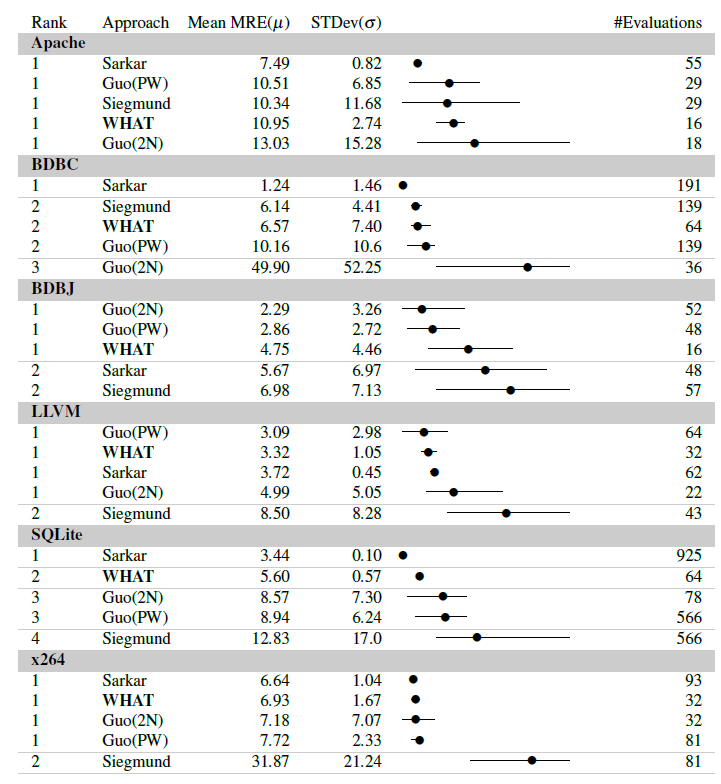
\includegraphics[width=\linewidth]{figures/OverviewPerformance}
	\caption{Overview and comparison over the mean error rate (mean MRE, $\mu$) and the standard deviation ($\sigma$) of the presented approaches. Siegmund stands for \AFID and Guo for \textit{Variablity aware performance prediction}. Sarkar's approach was not discussed in this paper.
		 \inlineQuote{[The column] Rank is computed using Scott-Knott, bootstrap 95\% confidence, and	A12 test.} \cite{FasterDiscoveryofFasterSystemConfigurationsSiegmund2017}}
	\label{fig:ConclusionPerformanceOverview}
\end{figure}
\FloatBarrier